% !TEX encoding = UTF-8 Unicode
% $Header: /cvsroot/latex-beamer/latex-beamer/solutions/conference-talks/conference-ornate-20min.en.tex,v 1.6 2004/10/07 20:53:08 tantau Exp $

\documentclass[handout]{beamer}
\usepackage{icomma}

% This file is a solution template for:

% - Talk at a conference/colloquium.
% - Talk length is about 20min.
% - Style is ornate.

\mode<presentation>
{
  \usetheme{Warsaw}
  % or ...

  \setbeamercovered{transparent}
  % or whatever (possibly just delete it)
  
  \setbeamertemplate{navigation symbols}{}
  
  \newcommand*\oldmacro{}%
  \let\oldmacro\insertshorttitle%
  \renewcommand*\insertshorttitle{%
    \oldmacro\hfill%
    \insertframenumber\,/\,\inserttotalframenumber}
}

\usepackage[utf8]{inputenc}
% or whatever

\usepackage{times}
\usepackage{multirow}
\usepackage[T1]{fontenc}
\usepackage{graphicx}
\usepackage{eso-pic}
\usepackage{color}
\usepackage{tikz}
\usepackage{wasysym}

% Or whatever. Note that the encoding and the font should match. If T1
% does not look nice, try deleting the line with the fontenc.

\title[]
{New Insights in Preference Elicitation\\for Recommender Systems}

\author[]
{Jill-Jênn Vie\\[5mm]\footnotesize iSWAG Symposium 2016}

\institute[]
{\includegraphics[width=0.5\linewidth]{figures/mangaki.png}}

\date
{June 10, 2016}

\begin{document}

\definecolor{vert}{rgb}{0.07 0.54 0.07}

{
\setbeamertemplate{headline}[default]
\begin{frame}
	\titlepage
\end{frame}
}

\def\R{\mathcal{R}}
\def\N{N}

\begin{frame}
	\frametitle{Mangaki}
    \includegraphics[width=\linewidth]{figures/ratings.jpg}
	\begin{itemize}
	\item 2k users
	\item 14k works (anime \& manga)
	\item 281k ratings (like / dislike / neutral / willsee / wontsee)
	\item October 2015: Student Demo Cup winner, Microsoft prize
	\item February 2016: Japanese Culture Embassy Prize, Paris
	\end{itemize}
\end{frame}

\begin{frame}
	\frametitle{Collaborative Filtering}
	\begin{block}{Problem}
		\begin{itemize}[<+->]
		\item Users $u = 1, \ldots, n$ and items $i = 1, \ldots, m$
		\item Every user $u$ rates some items $\R_u$\\(\alert{$r_{ui}$}: rating of user $u$ on item $i$)
        \item How to guess unknown ratings?
		\end{itemize}
	\end{block}
	\pause
	\begin{exampleblock}{$k$-nearest neighbor}
        \begin{itemize}
        \item Similarity score between users:
        \[ score(u, v) = \frac{\R_u \cdot \R_v}{||\R_u|| \cdot ||\R_v||}. \]
        \item Let's find user's $k$ nearest neighbors
        \item And recommend what they liked that he didn't rate
        \end{itemize}
	\end{exampleblock}
	Objects: $n$ vectors over $m$ dimensions
\end{frame}

\begin{frame}
    \frametitle{Preference Elicitation}
    \begin{block}{Problem}
        What questions to ask adaptively to a new user?
    \end{block}
    \pause
    \begin{exampleblock}{4 decks}
        \begin{itemize}
        \item Popularity
        \item Controversy (Reddit)
        \[ controversy(L, D) = {(L + D)}^{min(L / D, D / L)} \]
        \item Most liked
        \item Precious pearls: few rates but almost no dislike
        \end{itemize}
    \end{exampleblock}
    Problem: most people can't rate the controversial items
\end{frame}

\begin{frame}
	\frametitle{Matrix Completion}
	Let us assume that $M$ has \alert{low rank} $r$ :
	\[ M = \left(\begin{array}{c}
	\R_1\\
	\R_2\\
	\vdots\\
	\R_n
	\end{array}\right) = \raisebox{-1cm}{\begin{tikzpicture}
	\draw (0,0) rectangle (2.5,2);
	\end{tikzpicture}} =
	\raisebox{-1cm}{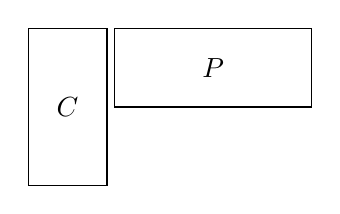
\begin{tikzpicture}
	\draw (0,0) rectangle ++(1,2);
	\draw node at (0.5,1) {$C$};
	\draw (1.1,1) rectangle ++(2.5,1);
	\draw node at (2.35,1.5) {$P$};
	\end{tikzpicture}} \]
	Every line $\R_u$ is a linear combination of lines of $P$.
	\centering
	$\visible<2->{M : \alert{n} \times \alert{m}} \qquad \visible<3->{C : \alert{n} \times \alert{r}} \qquad \visible<4->{P : \alert{r} \times \alert{m}.}$
	\visible<5->{$\R_1 = c_{11} P_1 + c_{12} P_2 + \ldots + c_{1r} P_r \qquad C_1 = (c_{11}, c_{12}, \ldots, c_{1r})$}
	\visible<6->{\begin{exampleblock}{Example}
	\begin{tabular}{@{}lccc@{}}
	If $P$ & $P_1$ : adventure & $P_2$ : romance & $P_3$ : plot twist\\
	And $C_u$ & $0,2$ & $-0,5$ & $0,6$
	\end{tabular}\\
	it means :\\
	\centering \small $u$ \alert{likes a bit} adventure, \alert{dislikes} romance,\\
	\alert{really likes} plot twists.
	\end{exampleblock}}
\end{frame}

\begin{frame}
    \frametitle{First Eigenvector's Top 30}
    \begin{columns}
    \begin{column}{0.5\textwidth}
  Nausicaä of the Valley of the Wind\\
                  Princesse Mononoké\\
             Le Château dans le ciel\\
                Le Voyage de Chihiro\\
               Toki wo Kakeru Shoujo\\
          Tengen Toppa Gurren Lagann\\
                            Baccano!\\
                        Cowboy Bebop\\
     Les Enfants Loups : Ame \& Yuki\\
          Mahou Shoujo Madoka Magica\\
          Suzumiya Haruhi no Yuuutsu\\
                         Porco Rosso\\
                         Summer Wars\\
             Neon Genesis Evangelion\\
                   Mon voisin Totoro\\
    \end{column}
    \begin{column}{0.5\textwidth}
                  Ghost in the Shell\\
             Kiki la petite sorcière\\
       Suzumiya Haruhi no Shoushitsu\\
                 Le Château ambulant\\
                             Paprika\\
                 The Garden of Words\\
                           Barakamon\\
                         Steins\string;Gate\\
           5 centimètres par seconde\\
              Grave of the Fireflies\\
     The Tale of The Princess Kaguya\\
                               Akira\\
                            Mushishi\\
                      Bakemonogatari\\
                          Durarara!!
    \end{column}
    \end{columns}
\end{frame}

\begin{frame}
    \frametitle{First Eigenvector's Bottom 30}
    \begin{columns}
    \begin{column}{0.5\textwidth}
                                   Zero no Tsukaima\\
                                         To LOVE-Ru\\
                                         Soul Eater\\
                                         D.Gray-man\\
                                            Another\\
                                             Bleach\\
                           Rosario to Vampire Capu2\\
                                     Vampire Knight\\
                                    High School DxD\\
                                             Naruto\\
                                       Black Butler\\
                                     Dragon Ball GT\\
                                       Guilty Crown\\
                                     Akame ga Kill!\\
   Naruto the Movie 2: Legend of the Stone of Gelel\\
    \end{column}
    \begin{column}{0.5\textwidth}
                                        Mirai Nikki\\
                                        Tokyo Ghoul\\
                                 Rosario to Vampire\\
                               L'Attaque des Titans\\
                               IS: Infinite Stratos\\
                                         Fairy Tail\\
                                Sword Art Online II\\
                                     Ao no Exorcist\\
                                          One Piece\\
                             Highschool of the Dead\\
                                   Sword Art Online\\
                                             Bleach\\
                                             Naruto\\
                                         Fairy Tail\\
                                 Naruto: Shippuuden\\
    \end{column}
    \end{columns}
\end{frame}

\begin{frame}
    \frametitle{Second Eigenvector's Top 30}
    \begin{columns}
    \begin{column}{0.5\textwidth}
                                L'Attaque des Titans\\
                    Fullmetal Alchemist: Brotherhood\\
                                          Death Note\\
                                 Fullmetal Alchemist\\
                                    Sword Art Online\\
                                Le Voyage de Chihiro\\
                                  Princesse Mononoké\\
                                      Ao no Exorcist\\
                                     No Game No Life\\
                                         Tokyo Ghoul\\
                                   Mon voisin Totoro\\
                                 FullMetal Alchemist\\
                                         Psycho-Pass\\
                             Attaque Des Titans (l')\\
                     Code Geass: Hangyaku no Lelouch\\
    \end{column}
    \begin{column}{0.5\textwidth}
                                              Naruto\\
                                           Fate/Zero\\
                      Les Enfants Loups : Ame \& Yuki\\
                                     Hunter x Hunter\\
     Fullmetal Alchemist: Brotherhood OVA Collection\\
                                         Mirai Nikki\\
                                          Death note\\
                                         Steins\string;Gate\\
                                          Soul Eater\\
                                           One Piece\\
                                 Le Château ambulant\\
                             Le Château dans le ciel\\
                                              Bleach\\
                                          Durarara!!\\
                                         Tokyo ghoul\\
    \end{column}
    \end{columns}
\end{frame}

\begin{frame}
    \frametitle{Second Eigenvector's Bottom 30}
    \begin{columns}
    \begin{column}{0.5\textwidth}
                                  Infinite Stratos 2\\
                                IS: Infinite Stratos\\
                          Ikkitousen: Dragon Destiny\\
                             The Severing Crime Edge\\
   IS: Infinite Stratos Encore - Koi ni Kogareru ...\\
                        A Bridge to the Starry Skies\\
                                       Sailor Moon R\\
                                         Ikki Tousen\\
                                  Vividred Operation\\
              School Days: Magical Heart Kokoro-chan\\
                            Papa to Kiss in the Dark\\
                                       D.C.~Da Capo~\\
                                          Rail Wars!\\
                                    Strawberry Panic\\
                                            Freezing\\
    \end{column}
    \begin{column}{0.5\textwidth}
                                          To LOVE-Ru\\
                                         School Days\\
                                       Tokyo Mew Mew\\
                            Haruka Nogizaka's Secret\\
                                                R-15\\
                                   Wizard Barristers\\
               Choujigen Game Neptune: The Animation\\
                                        Yu-Gi-Oh! GX\\
                                      Dragon Ball GT\\
                                       Captain Earth\\
                                     Astarotte's Toy\\
                                        Sakura Trick\\
                           Girls Bravo: First Season\\
                                          Kiss x Sis\\
                                            Dog Days\\
    \end{column}
    \end{columns}
\end{frame}

\begin{frame}
	\frametitle{Map}
	\includegraphics[width=\linewidth]{figures/map.png}
\end{frame}

\begin{frame}
	\frametitle{Map}
	\includegraphics[width=\linewidth]{figures/here.png}
\end{frame}

\begin{frame}
	\frametitle{Yahoo's Bootstrapping Decision Trees}
	\includegraphics[width=\linewidth]{figures/decisiontree.png}
\end{frame}

\begin{frame}
    \frametitle{Modelling Diversity: Determinantal Point Processes}
    \includegraphics[width=\linewidth]{figures/dpp.png}
\end{frame}

\begin{frame}
    \frametitle{Determinantal Point Processes}
    We want to sample over $n$ items\\
    $K : n \times n$ \alert{similarity matrix} over items\\(semidefinite positive matrix)\\
    $P$ is a \alert{determinantal point process} if $Y$ is drawn with property:
    \[ \forall A \subset Y, \quad P(A \subseteq Y) \propto det(K_A) \]
    \begin{example}
    \begin{columns}
    \begin{column}{0.5\textwidth}
    \[ K = \left(\begin{array}{cccc}
    1 & 2 & 3 & 4\\
    2 & 5 & 6 & 7\\
    3 & 6 & 8 & 9\\
    4 & 7 & 9 & 1
    \end{array}\right) \]
    \end{column}
    \begin{column}{0.5\textwidth}
    $A = \{1, 2, 4\}$ will be included with probability prop. to
    \[ K_A = det\left(\begin{array}{ccc}
    1 & 2 & 4\\
    2 & 5 & 7\\
    4 & 7 & 1
    \end{array}\right) \]
    \end{column}
    \end{columns}
    \end{example}
\end{frame}

\begin{frame}
    \frametitle{Link with diversity}
    \centering
    \includegraphics[width=0.7\linewidth]{figures/vol.png}
    \begin{itemize}
    \item The determinant is the volume of the vectors
    \item Non-correlated (\alert{diverse}) vectors will increase the volume
    \end{itemize}
    \begin{itemize}
    \item Algorithm samples with complexity $O(nk^3)$\\where $k$ is the number of points that will be sampled.
    \end{itemize}
\end{frame}

\begin{frame}
	\frametitle{Thanks for listening!}
	\includegraphics[width=\linewidth]{figures/mangaki.png}
	\vspace{5mm}
	\begin{columns}
	\begin{column}{0.5\textwidth}
	\begin{itemize}
	\item research.mangaki.fr\bigskip\\
	\item jj@mangaki.fr
	\end{itemize}\bigskip
	\end{column}
	\begin{column}{0.5\textwidth}
	\centering
	\huge Fork us\\on GitHub\!!
	\end{column}
	\end{columns}
	
	% \small (P. S. -- C'est la Code Week, apprenez à coder et tentez le concours \alert{figures/Prologin.org}, c'est gratuit et sans obligation d'achat !)
\end{frame}

\end{document}